\subsubsection{Software Architecture Requirements} \label{software_requirements}

Figure \ref{fig_design} illustrates the generic software architecture of the artifacts.
Each instantiated element adheres to the Element Naming Convention outlined in Appendix
\ref{appendix_element_naming_convention}. The following sections detail the requirements
specific to each element.

\begin{figure}[H]
    \centering
    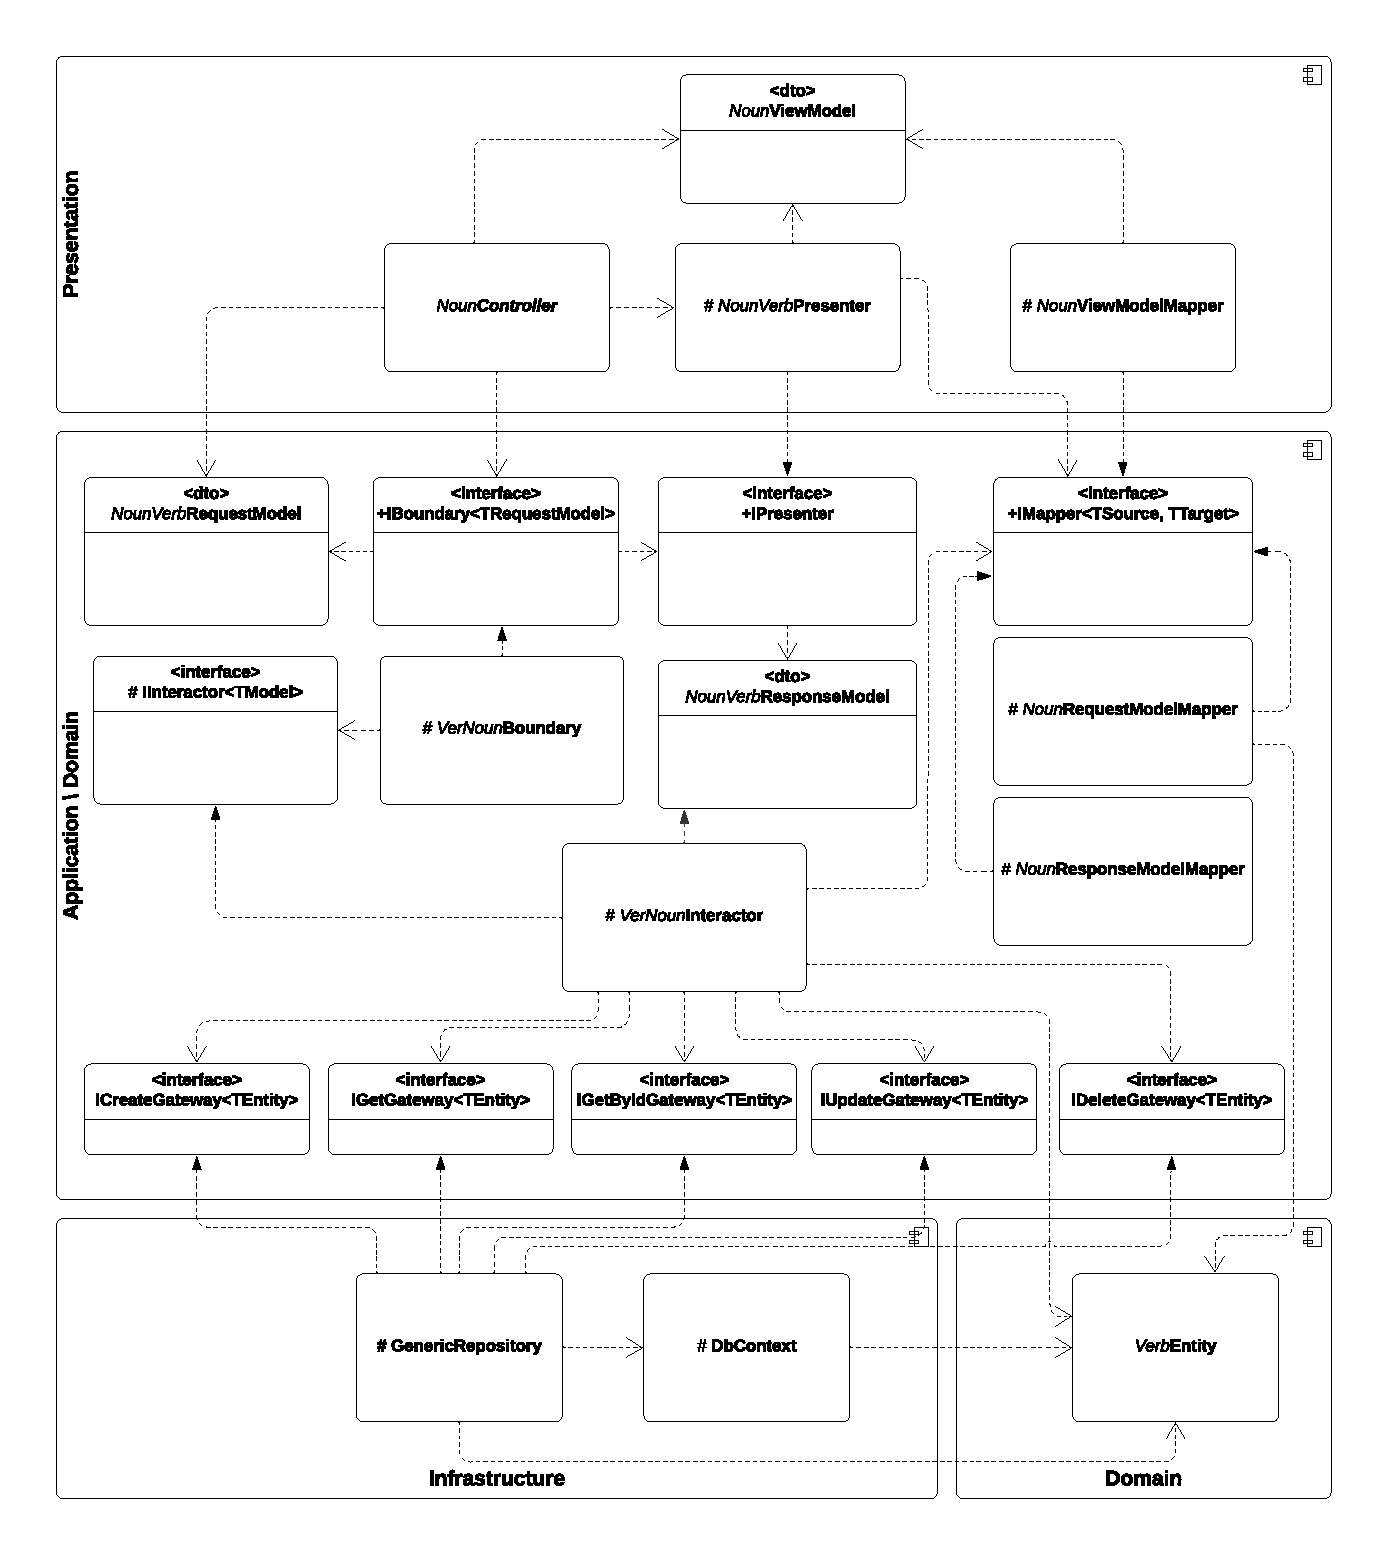
\includegraphics[width=0.4\textwidth]{figures/generic_design.pdf}
    \caption[Generic architecture]{The Generic architecture of the artifacts}
    \label{fig_design}
\end{figure}

requirement{The ViewModel}
\begin{enumerate}[label=\themycounter.\arabic*]
    \item The ViewModel consists of data attributes representing fields from the
    corresponding Entity. In addition, it may contain information specific to the user
    interface.
    \item The ViewModel has no external dependencies on other objects within the
    architecture.
\end{enumerate}

\requirement{The Presenter}
\begin{enumerate}[label=\themycounter.\arabic*]
    \item The Presenter Implementation is derived from the IPresenter interface and
    follows the specified implementation. The IPresenter interface can be found in the
    Application layer.
    \item The Presenter is responsible for creating the Controller's Response by
    instantiating the ViewModel, constructing the HTTP Response message, or combining both
    elements as needed.
    \item When required, the Presenter utilizes the IMapper interface without depending on
    specific implementations of the IMapper interface.
    \item The Presenter has an internal scope and cannot be instantiated outside the
    Presentation layer.
\end{enumerate}

\requirement{The ViewModelMapper}
\begin{enumerate}[label=\themycounter.\arabic*]
    \item The ViewModelMapper is derived from the IMapper interface and follows the
    specified implementation. The IMapper interface can be found in the Application layer.
    \item The ViewModelMapper is responsible for mapping the values of the necessary data
    attributes from the ResponseModel to the ViewModel.
    \item The ViewModelMapper has an internal scope and cannot be instantiated outside the
    Presentation layer.
\end{enumerate}

\requirement{The Controller}
\begin{enumerate}[label=\themycounter.\arabic*]
    \item The Controller is responsible for receiving external requests and forwarding the
    request to the appropriate Boundary within the Application layer.
    \item The Controller relies on the IBoundary interface without depending on specific
    implementations of the IBoundary interface.
\end{enumerate}

\requirement{The IBoundary}
\begin{enumerate}[label=\themycounter.\arabic*]
    \item The IBoundary interface establishes the contract for its derived Boundary
    implementations.
    \item The IBoundary interface has public scope within the system.
\end{enumerate}

\requirement{The Boundary Implementation}
\begin{enumerate}[label=\themycounter.\arabic*]
    \item A Boundary implementation is derived from the IBoundary interface and follows
    the specified implementation.
    \item The Boundary implementation separates the internal aspects of the Application
    Layer and the other layers within the component.
    \item Each Boundary implementation handles a single task, executed using the
    IInteractor interface.
    \item Boundary implementations have an internal scope and cannot be instantiated
    outside the Application layer.
\end{enumerate}

\requirement{The IInteractor}
\begin{enumerate}[label=\themycounter.\arabic*]
    \item The IInteractor interface establishes the contract for its derived Interactor
    implementations.
    \item The IInteractor has an internal scope and cannot be implemented outside the
    Application layer.
\end{enumerate}

\requirement{The Interactor Implementation}
\begin{enumerate}[label=\themycounter.\arabic*]
    \item An Interactor implementation is derived from the IInteractor interface and
    follows the specified implementation.
    \item The Interactor implementation executes a single task or orchestrates a series of
    tasks. Each of these tasks is implemented in separate Interactors. Alternatively, a
    Gateway is used for Tasks with Infrastructure dependencies, such as data persistence
    in a database.
    \item Depending on the task, the Interactor implementation orchestrates the mapping
    from RequestModels to Entities or from Entities to ResponseModels, utilizing the
    IMapper interface.
    \item Interactor implementations have an internal scope and cannot be implemented
    outside the Application layer.
\end{enumerate}

\requirement{The IMapper}
\begin{enumerate}[label=\themycounter.\arabic*]
    \item The IMapper interface establishes the contract for its derived Mapper
    implementations.
    \item The IMapper interface has a public scope within the system.
\end{enumerate}

\requirement{The RequestModelMapper}
\begin{enumerate}[label=\themycounter.\arabic*]
    \item The RequestModelMapper is derived from the IMapper interface and follows the
    specified implementation.
    \item The RequestModelMapper is responsible for mapping the values of the necessary
    data attributes from the RequestModel to an Entity.
    \item The RequestModelMapper has an internal scope and cannot be implemented outside
    the Application layer.
\end{enumerate}

\requirement{The ResponseModelMapper}
\begin{enumerate}[label=\themycounter.\arabic*]
    \item The RequestModelMapper is derived from the IMapper interface and follows the
    specified implementation.
    \item The RequestModelMapper is responsible for mapping the values of the necessary
    data attributes from the RequestModel to an Entity.
    \item The RequestModelMapper has an internal scope and cannot be implemented outside
    the Application layer.
\end{enumerate}

\requirement{The IPresenter}
\begin{enumerate}[label=\themycounter.\arabic*]
    \item The IPresenter interface establishes the contract for its derived Presenter
    implementations, typically implemented as part of the Presentation layer.
    \item The IPresenter interface has a public scope within the system.
\end{enumerate}

\requirement{The Gateway}
\begin{enumerate}[label=\themycounter.\arabic*]
    \item The Domain and Application layers have no dependencies on infrastructure
    technologies, like web- or database technologies.
    \item The \textit{[Verb]Gateway} interface establishes the contract for its derived
    Gateway implementations, typically implemented in the Infrastructure layer.
    \item The \textit{[Verb]}Gateway interface has a public scope within the system.
    \item Each task is represented in the naming convention of the interface. For example,
    the basic CRUD actions result in five IGateway interfaces:  ICreateGateway,
    IGetGateway, IGetByIdGateway, IUpdateGateway, and IDeleteGateway.
\end{enumerate}

\requirement{The ResponseModel}
\begin{enumerate}[label=\themycounter.\arabic*]
    \item The ResponseModel consists primarily of data attributes representing the fields
    of the corresponding Entity. Additionally, the ResponseModel may contain data specific
    to the output of the Interactor.
    \item The ResponseModel does not depend on external objects within the architecture.
\end{enumerate}

\requirement{The RequestModel}
\begin{enumerate}[label=\themycounter.\arabic*]
    \item The RequestModel consists primarily of data attributes representing the fields
    of the corresponding Entity. Additionally, the RequestModel may contain data specific
    to the input of the Interactor.
    \item The RequestModel does not depend on external objects within the architecture.
\end{enumerate}

\requirement{The Data Entity}
\begin{enumerate}[label=\themycounter.\arabic*]
    \item The Data Entity consists solely of attributes representing the corresponding
    data fields.
    \item The Data Entity does not rely on external objects within the architecture.
    \item The Application layer is the only layer that utilizes the Data Entity.
\end{enumerate}

\requirement{The Gateway Implementation}
\begin{enumerate}[label=\themycounter.\arabic*]
    \item The [\textit{Verb}]Gateway Implementation derives from the
    I[\textit{Verb}]Gateway interface and adheres to the specified implementation.
    \item The [\textit{Verb}]Gateway Implementation is responsible for the interaction
    associated with the specific task, utilizing the infrastructure technology of the
    specific layer (e.g., a SQL database or a filesystem).
    \item The [\textit{Verb}]Gateway Implementation has an internal scope and cannot be
    instantiated outside the layer.
\end{enumerate}

\requirement{The Design Principles}
\begin{enumerate}[label=\themycounter.\arabic*]
    \item Each architectural pattern adheres to at least one of the SOLID principles to
    ensure that none of the implementations violate these principles.
\end{enumerate}
